%! Author = itgramic
%! Date = 24.11.23

% Preamble
\chapter{Einführung}
{\color{black}Im Rahmen des von Microsoft indizierten Patchdays, bei dem Microsoft alle 2 Monate einen Patch veröffentlicht, müssen auch die \Gls{JBoss}-Server des KIS Phoenix angefasst werden.}

{\color{black} Das KIS Phoenix verfügt dabei über 4 JBoss-Server, 2 für die Testsysteme resp.
das Demosytsem und 2 für das produktive System.}
\begin{figure}[H]
    \centering
    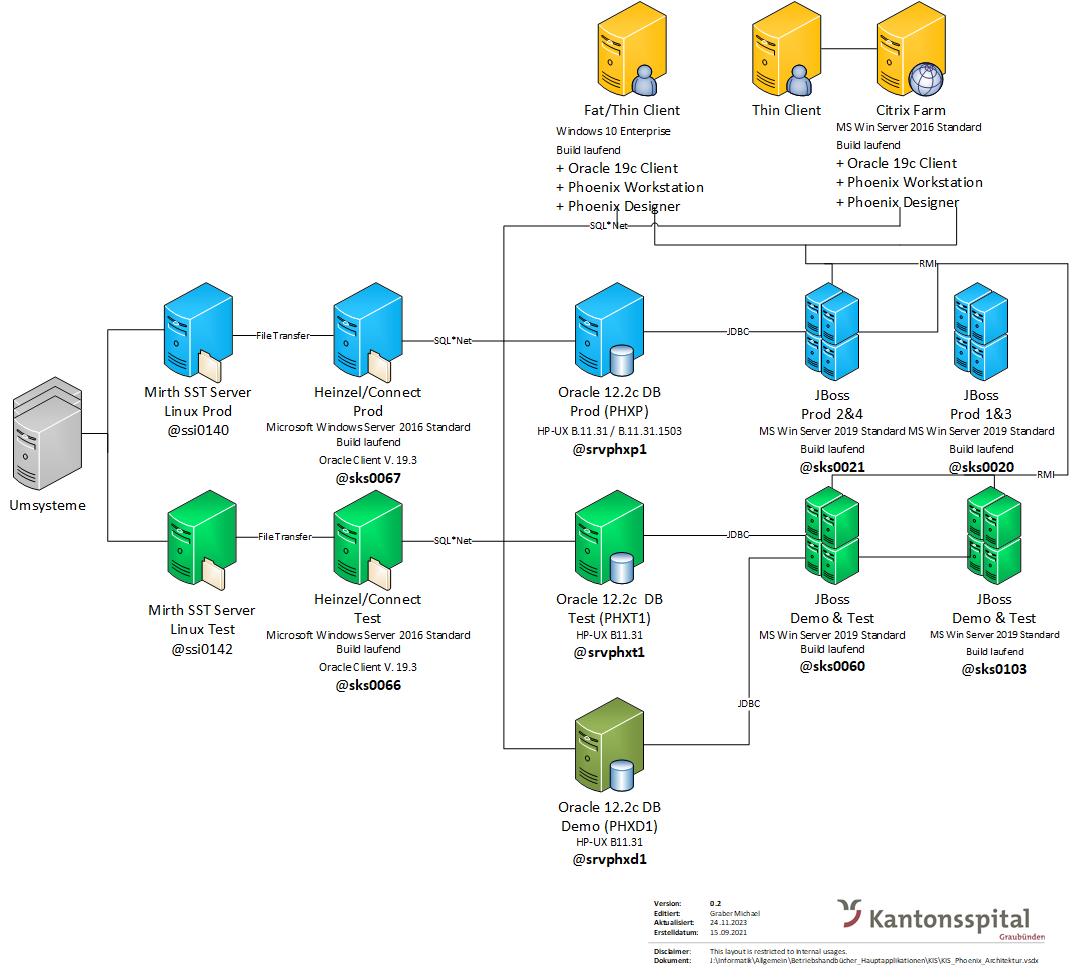
\includegraphics[width=1\linewidth]{source/introduction/KIS_Phoenix_Architektur}
    \caption{Architektur KIS Phoenix\cite{KFDFYH5H}}
    \label{fig:architektur-kis-phoenix}
\end{figure}
{\color{black}
Das Test1 und Demosystem hat je einen JBoss-Node auf einer Seite, das Test2 hat nur einen Node.
Das Produktivsystem hat je Site einen Node, also insgesamt vier Nodes.}

Die genaue Konfiguration sieht wie folgt aus:
% Please add the following required packages to your document preamble:
% \usepackage{booktabs}
% \usepackage{graphicx}
% \usepackage{lscape}
\begin{landscape}
\begin{table}[]
\centering
\resizebox{\columnwidth}{!}{%
\begin{tabular}{@{}lccccccccccc@{}}
\toprule
\textbf{Typ}                                                     & \textbf{Applikationsserver} & \textbf{}                & \textbf{}                & \textbf{}                & \multicolumn{5}{c}{}                                                                                                                      & \multicolumn{2}{c}{\textbf{Schnittstellenserver}} \\ \midrule
\textbf{\begin{tabular}[c]{@{}l@{}}Systeme\\ Rolle\end{tabular}} & \multicolumn{2}{c}{\textbf{Produktion}}                & \multicolumn{2}{c}{\textbf{Produktion}}             & \multicolumn{5}{c}{Test- und Demosystem Test- und Demosystem}                                                                             & \textbf{Produktion}        & \textbf{Test}        \\ \midrule
\multicolumn{1}{l|}{\textbf{Physikalischer Hostname}}            & \multicolumn{2}{c}{sks0020}                            & \multicolumn{2}{c}{sks0021}                         & \multicolumn{3}{c}{sks0060}                                                       & \multicolumn{2}{c}{sks0103}                           & sks0067                    & sks0066              \\
\multicolumn{1}{l|}{\textbf{IP Adresse phy. Host}}               & \multicolumn{2}{c}{10.0.22.43}                         & \multicolumn{2}{c}{10.0.22.44}                      & \multicolumn{3}{c}{10.0.22.52}                                                    &                           & 10.0.22.15                & 10.0.22.54                 & 10.0.22.53           \\
\multicolumn{1}{l|}{\textbf{IP Submask}}                         & \multicolumn{11}{c}{255.255.255.0}                                                                                                                                                                                                                                                                           \\
\multicolumn{1}{l|}{\textbf{Gateway}}                            & \multicolumn{11}{c}{10.0.22.1}                                                                                                                                                                                                                                                                               \\
\multicolumn{1}{l|}{\textbf{DNS 1}}                              & \multicolumn{11}{c}{10.0.16.163}                                                                                                                                                                                                                                                                             \\
\multicolumn{1}{l|}{\textbf{DNS 2}}                              & \multicolumn{11}{c}{10.0.16.163}                                                                                                                                                                                                                                                                             \\
\multicolumn{1}{l|}{\textbf{Timeserver}}                         & \multicolumn{11}{c}{10.10.146.196}                                                                                                                                                                                                                                                                           \\
\multicolumn{1}{l|}{\textbf{JBoss Nodes}}                        & prod1                       & prod3                    & prod2                    & prod4                    & demo11                    & test11                    & test21                    & demo12                    & test12                    &                            &                      \\
\multicolumn{1}{l|}{\textbf{Windows Services}}                   & PhoenixJBossEAP\_prod\_1    & PhoenixJBossEAP\_prod\_3 & PhoenixJBossEAP\_prod\_2 & PhoenixJBossEAP\_prod\_4 & PhoenixJBossEAP\_demo1\_1 & PhoenixJBossEAP\_test1\_1 & PhoenixJBossEAP\_test2\_1 & PhoenixJBossEAP\_demo1\_2 & PhoenixJBossEAP\_test1\_2 &                            &                      \\ \bottomrule
\end{tabular}%
}
\caption{Spezifikationen KIS Phoenix Applikations- und Schnittstellenserver}
\label{tab:kis-phoenix-server-specs}
\end{table}
\end{landscape}